\documentclass{beamer}

\usepackage{fontspec,xunicode,xltxtra}
\usepackage[french]{babel}
\usepackage{microtype}
\usepackage{default}	
\usepackage[]{hyperref}
\hypersetup{
	colorlinks=true,
	linkcolor=[rgb]{0.404,0.318,0.318},
	urlcolor=[rgb]{0.404,0.318,0.318}}
\usetheme{simple}
\usepackage{graphicx}
\usepackage[utf8]{inputenc}
\usepackage[justification=centering]{caption}
\usepackage{subcaption}
\usepackage{listings}
\usepackage{pstricks}
\setmainfont{Carlito}
\setsansfont{Carlito}
\setmonofont{Anonymous Pro Bold}
\captionsetup[subfigure]{labelformat=empty}
\captionsetup[figure]{labelformat=empty}
\setbeamertemplate{caption}{\raggedright\insertcaption\par}
\setbeamerfont{frametitle}{size=\LARGE}
\newfontfamily\DejaSans{DejaVu Sans}
\setbeamerfont{title}{family=\texttt,size=\huge}
\usepackage[scale=2]{ccicons}
\newfontfamily\unicodefun[Ligatures=TeX]{Symbola}

\title{i-score à l'horizon 2017}
\date{\today}
\author{Jean-Michaël Celerier}
\institute{LaBRI, Blue Yeti}

\newsavebox{\codebox}% For storing listings
\begin{document}
    
\maketitle

\begin{frame}
    \frametitle{En 2016}    
    \Large
    \begin{itemize}
    	\item Travail \textbf{spatial} $\rightarrow$ utilisation des formes cartésiennes pour définir des zones.
    	\item Travail sur \textbf{robots} $\rightarrow$ stages et protocoles.
    	\item Travail sur \textbf{audio} $\rightarrow$ fonctionnalités de séquenceur.
    \end{itemize}
\end{frame}

\begin{frame}
	\begin{columns}
		\begin{column}{0.5\textwidth}
			\begin{figure}
				\centering
			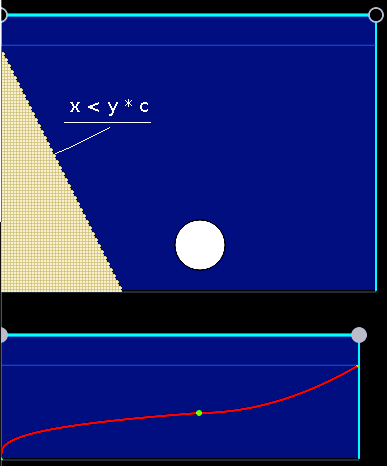
\includegraphics[width=0.9\textwidth]{images/arc1.png}	
			\end{figure}		
	    \end{column}
\begin{column}{0.5\textwidth}
	\begin{figure}
		\centering
		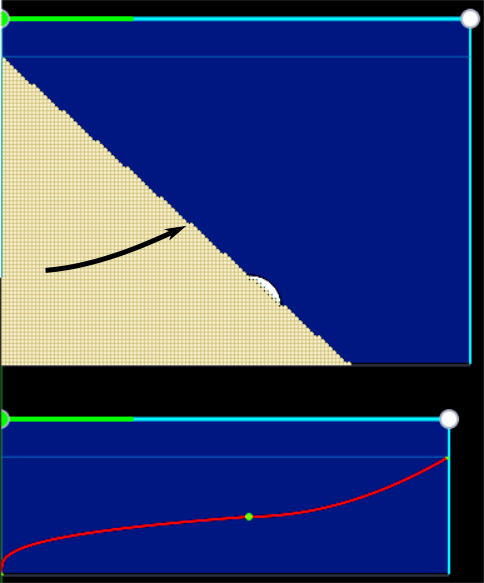
\includegraphics[width=0.9\textwidth]{images/arc3.png}	
	\end{figure}		
\end{column}
\end{columns}
\end{frame}

\begin{frame}
	\begin{figure}
		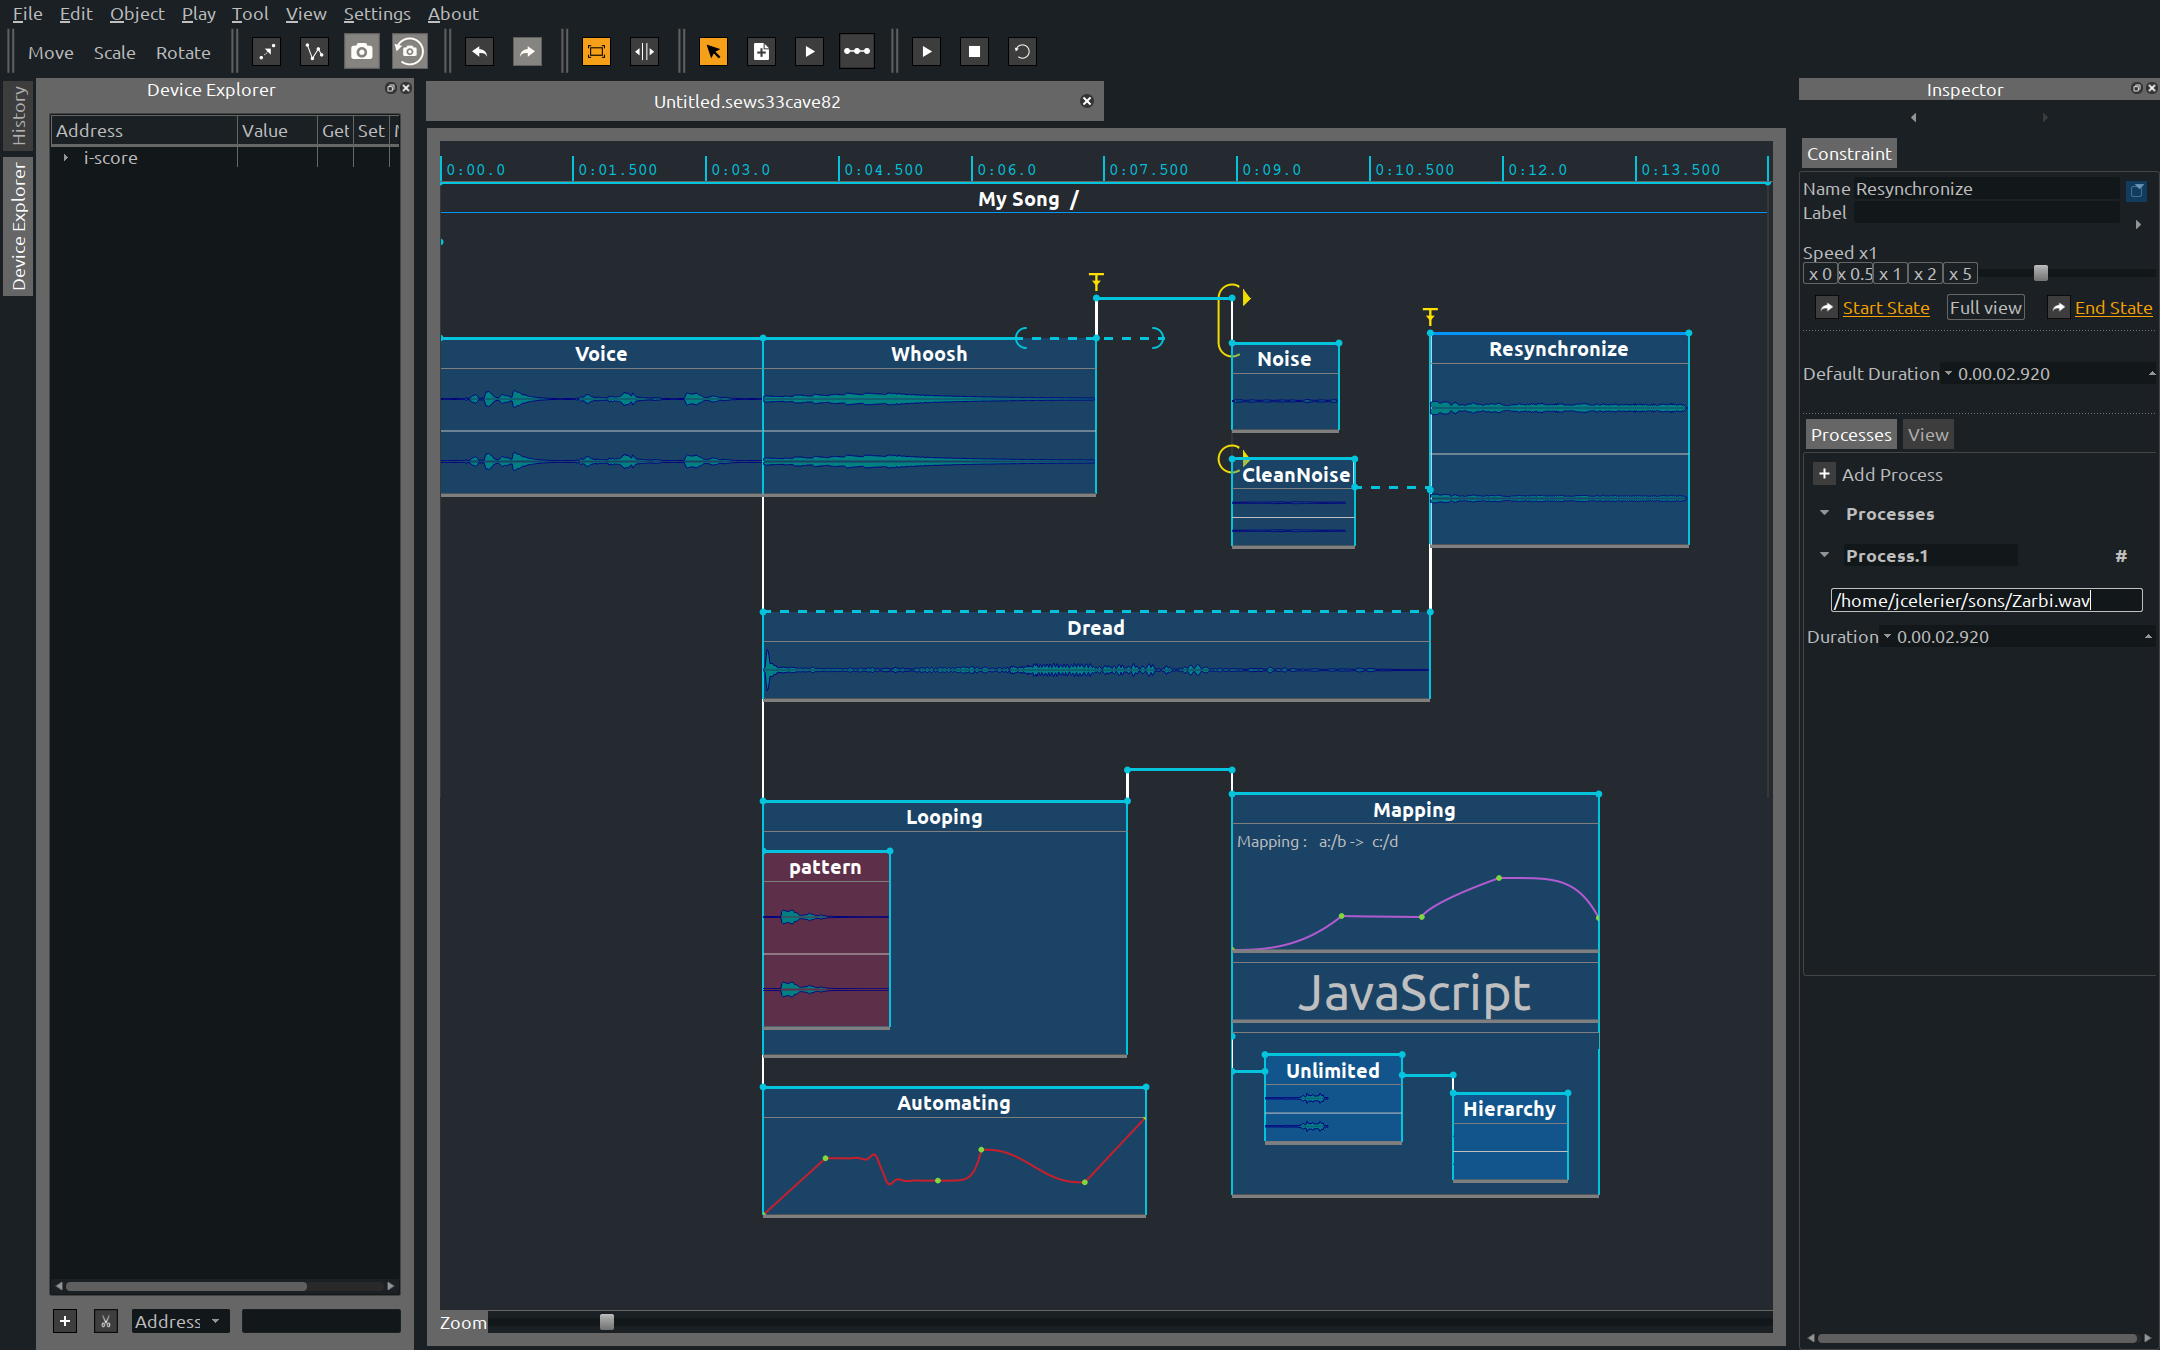
\includegraphics[width=\textwidth]{images/audio.png}
		\caption{Fonctionnalités audio}
	\end{figure}
\end{frame}

\begin{frame}
	\begin{figure}
		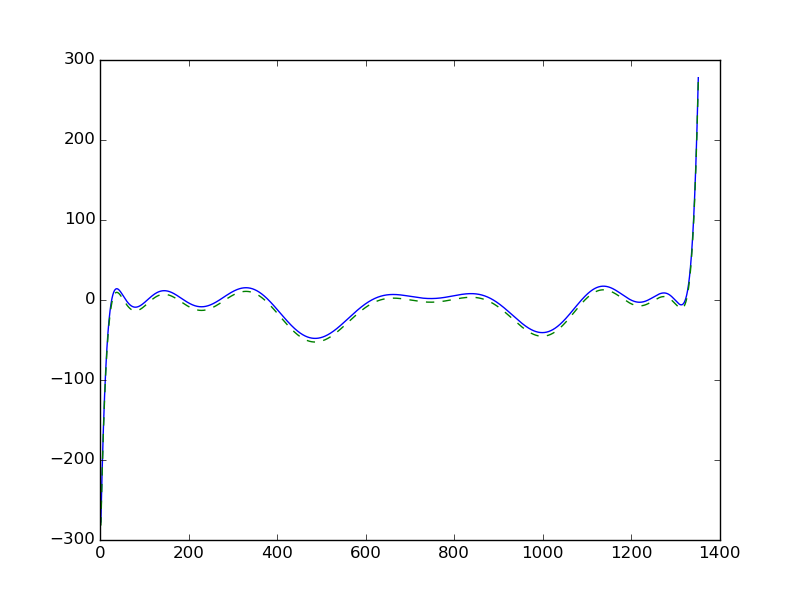
\includegraphics[width=0.25\textwidth]{images/graph/motor1.png}
		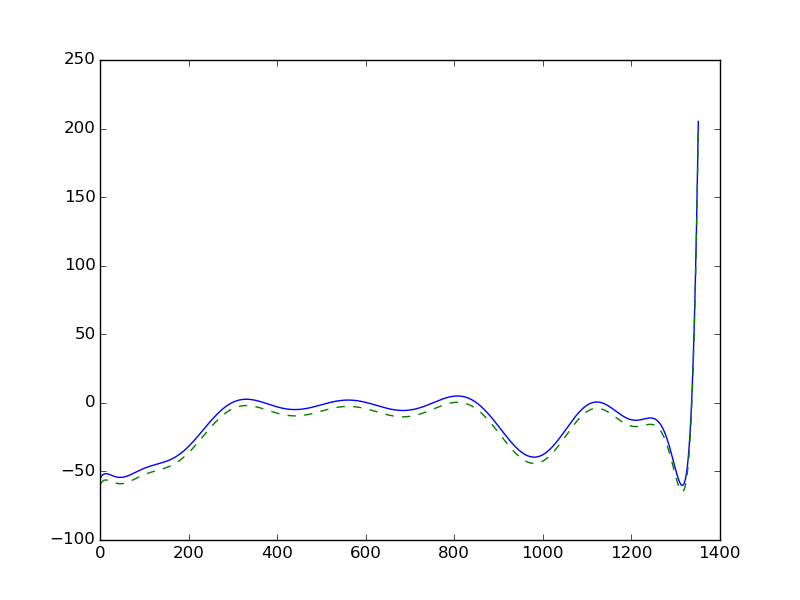
\includegraphics[width=0.25\textwidth]{images/graph/motor2.png}
		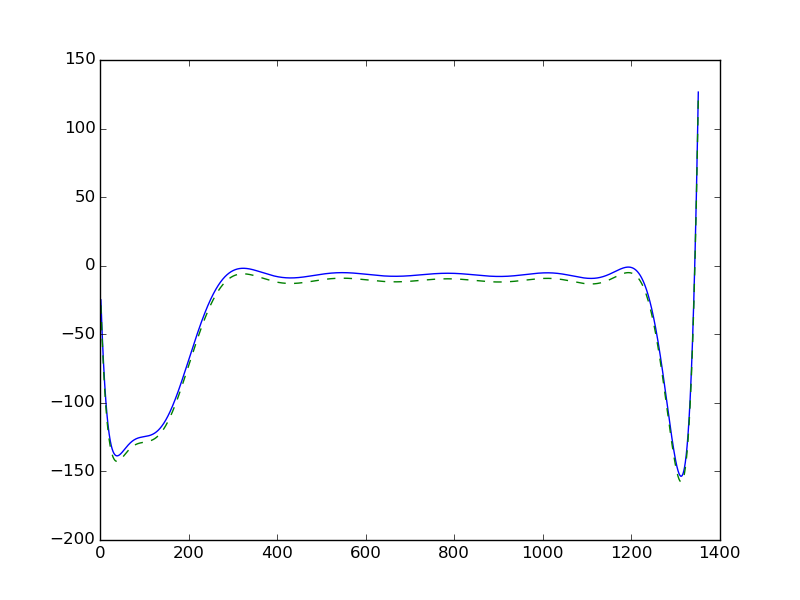
\includegraphics[width=0.25\textwidth]{images/graph/motor3.png}
		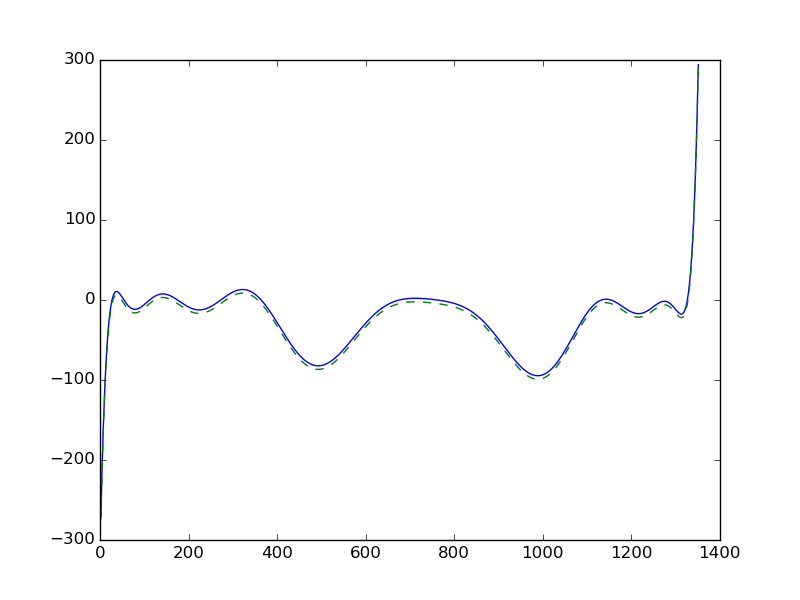
\includegraphics[width=0.25\textwidth]{images/graph/motor4.png}~\\
		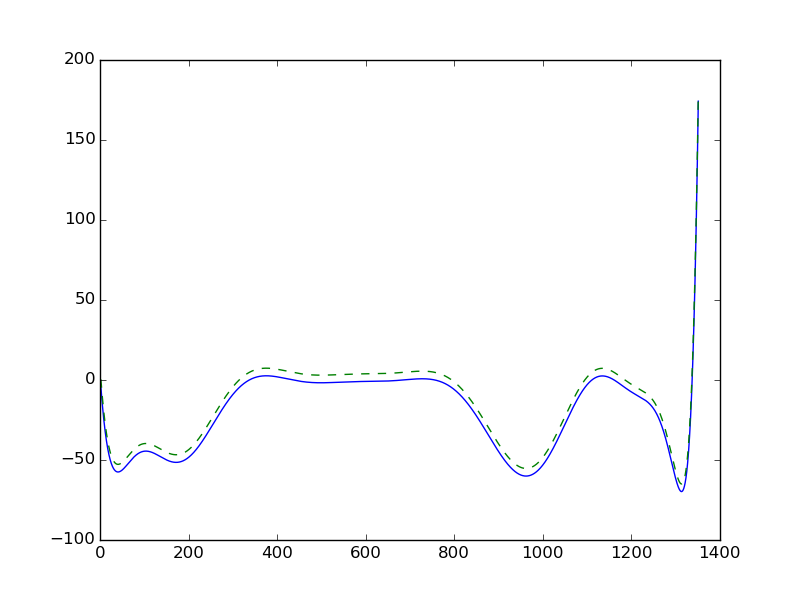
\includegraphics[width=0.25\textwidth]{images/graph/motor5.png}
		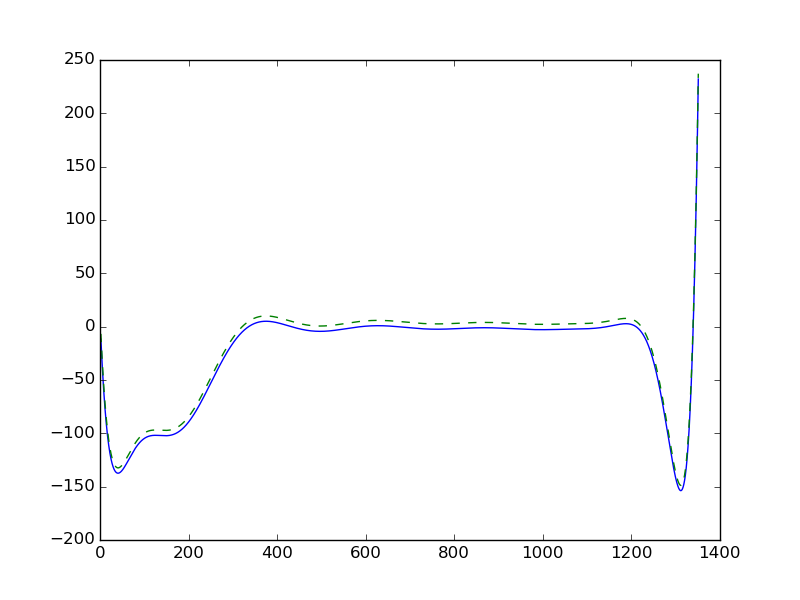
\includegraphics[width=0.25\textwidth]{images/graph/motor6.png}
		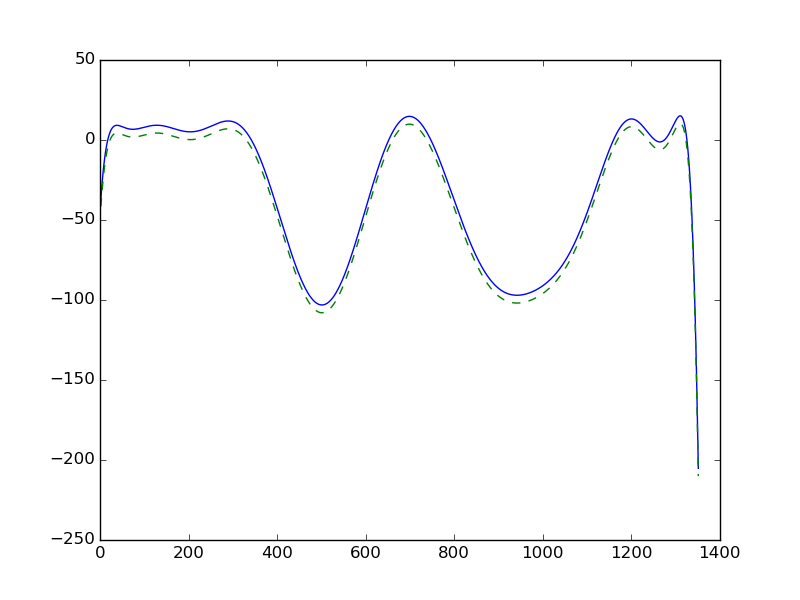
\includegraphics[width=0.25\textwidth]{images/graph/motor7.png}
		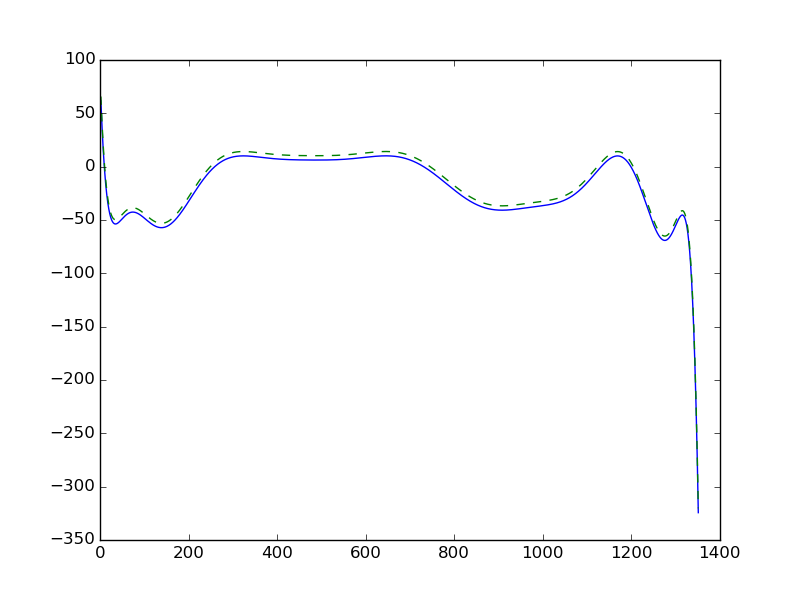
\includegraphics[width=0.25\textwidth]{images/graph/motor8.png}~\\
		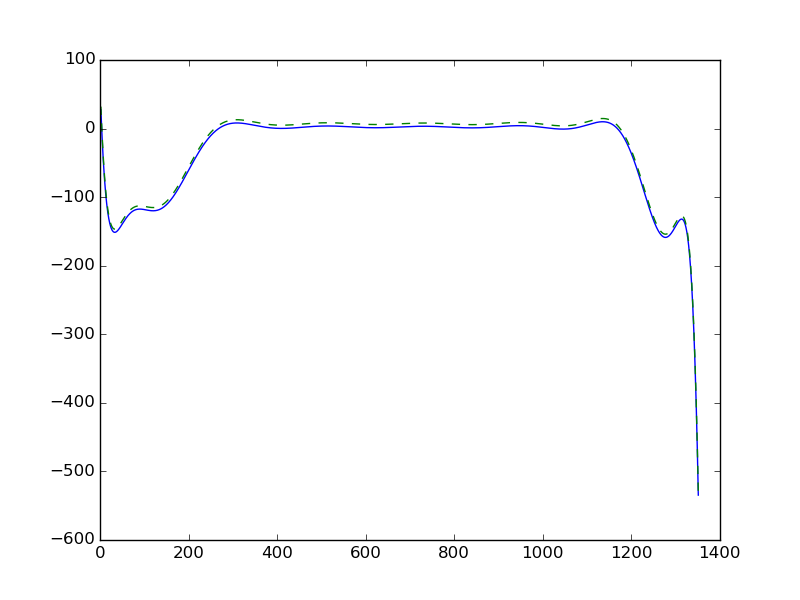
\includegraphics[width=0.25\textwidth]{images/graph/motor9.png}
		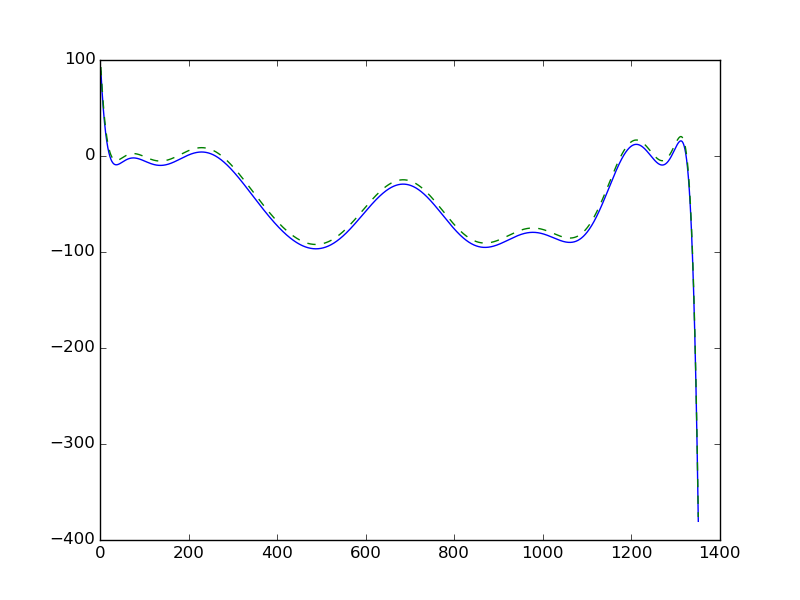
\includegraphics[width=0.25\textwidth]{images/graph/motor10.png}
		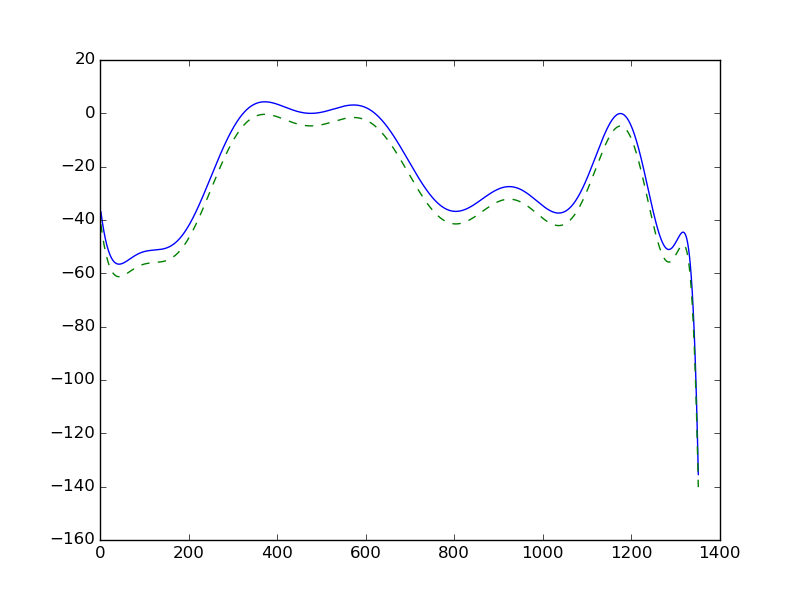
\includegraphics[width=0.25\textwidth]{images/graph/motor11.png}
		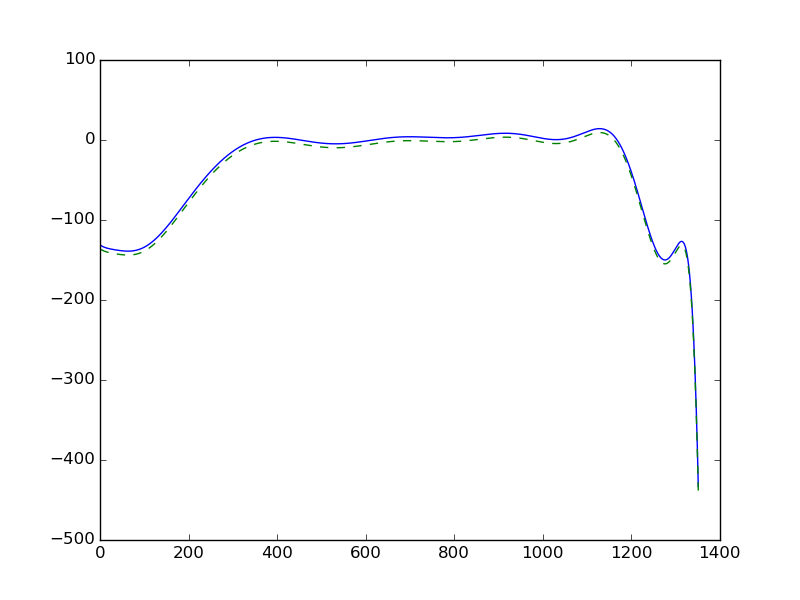
\includegraphics[width=0.25\textwidth]{images/graph/motor12.png}
		\caption{Mouvements des moteurs et interpolations (Maëva Grondin)}
	\end{figure}
\end{frame}
\begin{frame}
	\frametitle{À venir}    
	\Large
	\begin{itemize}
		\item En cours : typage des données manipulées.
		\begin{itemize}
			\item Implique la conception d'un modèle de calcul~: HSV $\rightarrow$ RGB $\rightarrow$ HSV.
		\end{itemize}
		~\\
		\item Problématique de la répartition.
		\begin{itemize}
			\item Implémentation de l'exécution sur plusieurs machines.
			\item Répartition des médias : flux A/V, scènes 3D\dots
			\item Répartition des programmes : on écrit un calcul dans PureData, et on incorpore une version pré-compilée dans le protocole pour exécution sur embarqué ou dans web.
		\end{itemize}
		
	\end{itemize}
\end{frame}

\begin{frame}
    \frametitle{Liens} 
    \Large
    \begin{itemize}
        \setlength\itemsep{1em}
        \item \textbf{Dépôt pour l'extension espace} :~\\
        \url{github.com/OSSIA/iscore-addon-space}
        \item \textbf{Dépôt pour l'extension audio} :~\\
        \url{github.com/OSSIA/iscore-addon-audio}
        \item \textbf{Dépôts pour le travail sur robots} :~\\
        \url{github.com/iscore-metabots}
        \item \textbf{Le logiciel} :~\\
         \url{i-score.org}
    \end{itemize}
        
    \centering
    \vspace{2em}
    \Large{Merci !}
\end{frame}    
\end{document}
